\begin{pastexam}[label={px:ccu-111-csb-02}]{中正資工所乙組 111 學年度 第 8 題}
（追蹤）

(22\%) Given the following numbers: 37, 5, 26, 1, 61, 11, 59, 15, 48, 19, please answer the following
questions.
\begin{enumerate}[label=(\alph*)]
\item (8\%) Please sort these numbers in ascending order with the following \texttt{quicksort} function in
C, where the \texttt{swap} function is used to swap two numbers. Note that the first number in each
sublist is always selected as the pivot, and you must show necessary steps such that \textbf{the use of
the \texttt{quicksort} function can be recognized}.
\item (7\%) Assume that the numbers are input sequentially. Please construct a binary search tree without
rotations.
\item (7\%) Please construct a max heap by adding the numbers \textbf{one by one}. Please do not directly
heapify it.
\end{enumerate}
\begin{minted}[fontsize=\small]{c}
void quicksort(int a[], int left, int right)
{
   int pivot, i, j;
   while (left < right) {
      i = left;
      j = right+1;
      pivot = a[left];
      do {
         do i++; while (a[i] < pivot);
         do j--; while (a[j] > pivot);
         if (i < j) swap(&a[i], &a[j]);
      } while (i < j);
      swap(&a[left], &a[j]);
      if ( j - left < right - j ) {
         quicksort(a, left, j-1);
         left = j + 1;
      }
      else {
         quicksort(a, j+1, right);
         right = j - 1;
      }
   }
}
\end{minted}
\end{pastexam}

\begin{pastsoln}
三個小題分屬資結書第~14、9、8~章；(a) 最吃重，放在本章。

\textbf{(a)} 先看程式在做什麼。 分割和資結書第~14.5~節的 Hoare 分割（虛擬碼~14.10）同一類：$i$ 從左往右找
$\ge \mathit{pivot}$ 的數，$j$ 從右往左找 $\le \mathit{pivot}$ 的數，$i < j$ 就交換；兩者交錯後把基準 $a[\mathit{left}]$ 和
$a[j]$ 對調，基準就定位在 $j$。 和一般寫法不同的是後半段：只對\textbf{比較短}的那一段遞迴呼叫，比較長的那一段改
\texttt{left} 或 \texttt{right} 之後由外層的 \texttt{while} 迴圈繼續處理（尾遞迴改成迴圈），所以遞迴深度最多
$O(\log n)$（資結書第~6.4~節）。 題目要求「看得出用了這個函式」，下面每一次分割都寫出範圍、交換、$j$，以及哪一段
遞迴、哪一段留給迴圈。 （內層的 \texttt{do i++} 沒有檢查邊界，要靠 $a[\mathit{right}+1] \ge \mathit{pivot}$ 擋住；這組
資料每次都擋得住，見下面 $[7..9]$ 那一步 $i$ 停在 $61$。）

陣列索引 $0$--$9$，一開始 $[37, 5, 26, 1, 61, 11, 59, 15, 48, 19]$，呼叫 \texttt{quicksort(a, 0, 9)}。
\begin{enumerate}[label=\arabic*.]
\item 範圍 $[0..9]$，pivot $= 37$。 $i$ 停在 $61$（索引 $4$），$j$ 停在 $19$（索引 $9$），交換；$i$ 停在 $59$（索引 $6$），
$j$ 停在 $15$（索引 $7$），交換；$i$ 停在索引 $7$（$59$），$j$ 停在索引 $6$（$15$），交錯。 $a[0]$ 和 $a[6]$ 對調：
\[
[15, 5, 26, 1, 19, 11, \underline{37}, 59, 48, 61], \qquad j = 6.
\]
左段 $[0..5]$ 有 $6$ 個、右段 $[7..9]$ 有 $3$ 個，$j - \mathit{left} = 6 < \mathit{right} - j = 3$ 不成立，走 else：遞迴
\texttt{quicksort(a, 7, 9)}，之後 $\mathit{right} = 5$。
  \begin{itemize}
  \item 遞迴 $[7..9] = [59, 48, 61]$，pivot $= 59$。 $i$ 跳過 $48$ 停在 $61$（索引 $9$），$j$ 停在 $48$（索引 $8$），沒有交換；
  $a[7]$、$a[8]$ 對調得 $[48, \underline{59}, 61]$，$j = 8$。 $1 < 1$ 不成立，遞迴 \texttt{quicksort(a, 9, 9)}（一個數，
  直接返回），$\mathit{right} = 7$，迴圈結束。 陣列：$[15, 5, 26, 1, 19, 11, 37, 48, 59, 61]$。
  \end{itemize}
\item 回到最外層，範圍 $[0..5] = [15, 5, 26, 1, 19, 11]$，pivot $= 15$。 $i$ 停在 $26$（索引 $2$），$j$ 停在 $11$（索引 $5$），
交換得 $[15, 5, 11, 1, 19, 26]$；$i$ 停在 $19$（索引 $4$），$j$ 停在 $1$（索引 $3$），交錯。 $a[0]$、$a[3]$ 對調：
\[
[1, 5, 11, \underline{15}, 19, 26, 37, 48, 59, 61], \qquad j = 3.
\]
$3 < 2$ 不成立，遞迴 \texttt{quicksort(a, 4, 5)}，之後 $\mathit{right} = 2$。
  \begin{itemize}
  \item 遞迴 $[4..5] = [19, 26]$，pivot $= 19$，$i$ 停在 $26$，$j$ 停在 $19$ 本身，$j = 4$，不變。 $0 < 1$，遞迴
  \texttt{quicksort(a, 4, 3)}（空的），$\mathit{left} = 5$，迴圈結束。
  \end{itemize}
\item 範圍 $[0..2] = [1, 5, 11]$，pivot $= 1$，$j$ 一路退到索引 $0$，$j = 0$，不變。 $0 < 2$，遞迴
\texttt{quicksort(a, 0, -1)}（空的），$\mathit{left} = 1$。
\item 範圍 $[1..2] = [5, 11]$，pivot $= 5$，$j = 1$，不變。 $0 < 1$，遞迴 \texttt{quicksort(a, 1, 0)}（空的），
$\mathit{left} = 2$，$\mathit{left} < \mathit{right}$ 不成立，結束。
\end{enumerate}
結果 $[1, 5, 11, 15, 19, 26, 37, 48, 59, 61]$。

\textbf{(b)} 依序插入，比節點小往左、大往右，走到空的位置放下（資結書第~9.2~節）：$37$ 當根；$5 < 37$ 左；
$26$：$37$ 左、$5$ 右；$1$：$5$ 的左；$61$：$37$ 右；$11$：$37 \to 5 \to 26$ 的左；$59$：$61$ 的左；$15$：$37 \to 5 \to 26
\to 11$ 的右；$48$：$61 \to 59$ 的左；$19$：$37 \to 5 \to 26 \to 11 \to 15$ 的右。
\begin{center}
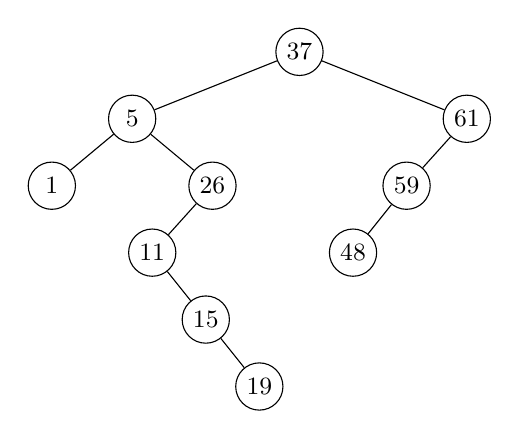
\begin{tikzpicture}[x=0.85cm,y=0.85cm,n/.style={circle,draw,inner sep=0pt,minimum size=6mm,font=\small}]
\node[n] (37) at (0,0) {37};
\node[n] (5) at (-2.5,-1) {5};   \node[n] (61) at (2.5,-1) {61};
\node[n] (1) at (-3.7,-2) {1};   \node[n] (26) at (-1.3,-2) {26}; \node[n] (59) at (1.6,-2) {59};
\node[n] (11) at (-2.2,-3) {11}; \node[n] (48) at (0.8,-3) {48};
\node[n] (15) at (-1.4,-4) {15};
\node[n] (19) at (-0.6,-5) {19};
\draw (37)--(5) (37)--(61) (5)--(1) (5)--(26) (26)--(11) (11)--(15) (15)--(19) (61)--(59) (59)--(48);
\end{tikzpicture}
\end{center}

\textbf{(c)} 一個一個插入：放在最後一格，再和父節點比，比父節點大就交換往上浮（資結書第~8.1~節、虛擬碼~8.2）。
用陣列表示（索引從 $1$ 起，$i$ 的父節點是 $\lfloor i/2 \rfloor$）：
\begin{center}
\begin{tabular}{lll}
\toprule
插入 & 上浮的過程 & 陣列 \\
\midrule
$37$ & & $[37]$ \\
$5$ & $5 < 37$ & $[37, 5]$ \\
$26$ & $26 < 37$ & $[37, 5, 26]$ \\
$1$ & $1 < 5$ & $[37, 5, 26, 1]$ \\
$61$ & 和 $5$、$37$ 交換 & $[61, 37, 26, 1, 5]$ \\
$11$ & $11 < 26$ & $[61, 37, 26, 1, 5, 11]$ \\
$59$ & 和 $26$ 交換，$59 < 61$ & $[61, 37, 59, 1, 5, 11, 26]$ \\
$15$ & 和 $1$ 交換，$15 < 37$ & $[61, 37, 59, 15, 5, 11, 26, 1]$ \\
$48$ & 和 $15$、$37$ 交換，$48 < 61$ & $[61, 48, 59, 37, 5, 11, 26, 1, 15]$ \\
$19$ & 和 $5$ 交換，$19 < 48$ & $[61, 48, 59, 37, 19, 11, 26, 1, 15, 5]$ \\
\bottomrule
\end{tabular}
\end{center}
最後的最大堆積：
\begin{center}
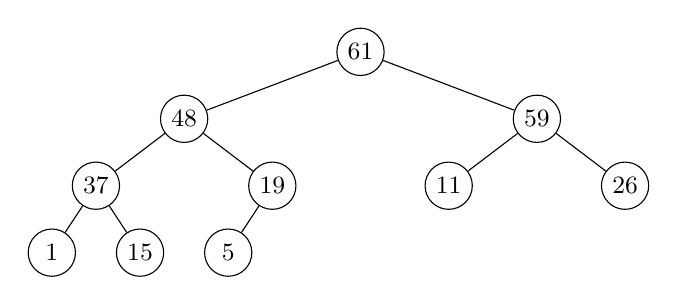
\begin{tikzpicture}[x=0.8cm,y=0.85cm,n/.style={circle,draw,inner sep=0pt,minimum size=6mm,font=\small}]
\node[n] (a) at (0,0) {61};
\node[n] (b) at (-2.8,-1) {48};  \node[n] (c) at (2.8,-1) {59};
\node[n] (d) at (-4.2,-2) {37};  \node[n] (e) at (-1.4,-2) {19};
\node[n] (f) at (1.4,-2) {11};   \node[n] (g) at (4.2,-2) {26};
\node[n] (h) at (-4.9,-3) {1};   \node[n] (i) at (-3.5,-3) {15};  \node[n] (j) at (-2.1,-3) {5};
\draw (a)--(b) (a)--(c) (b)--(d) (b)--(e) (c)--(f) (c)--(g) (d)--(h) (d)--(i) (e)--(j);
\end{tikzpicture}
\end{center}
\end{pastsoln}
